\chapter{Arhitektura i dizajn sustava}
		
		%\textbf{\textit{dio 1. revizije}}\\

		%\textit{ Potrebno je opisati stil arhitekture te identificirati: podsustave, preslikavanje na radnu platformu, spremišta podataka, mrežne protokole, globalni upravljački tok i sklopovsko-programske zahtjeve. Po točkama razraditi i popratiti odgovarajućim skicama:}
	\begin{itemize}
		\item 	%\textit{izbor arhitekture temeljem principa oblikovanja pokazanih na predavanjima (objasniti zašto ste baš odabrali takvu arhitekturu)}
		Aplikacija se sastoji od backend-a, frontend-a i baze podataka. \newline Backend je pozadinski dio aplikacije koji se izvršava na serveru. Za razvoj backend-a odabran je programski jezik Java i okvir Spring što čini backend prenosiv i jednostavan za korištenje. Sastoji se od rest kontrolera koji primaju HTTP zahtjeve i vraćaju JSON podatke, Service komponenti koje provjeravaju točnost upita i valjanost njihovih vrijednosti te konačno Repository komponenti koji omogućuju upisivanje u bazu i čitanje iste. \newline Frontend je grafičko sučelje koje omogućuje prijavu u aplikaciju, prikaz traženih podataka te lakše korištenje aplikacije. Za razvoj frontend-a odabran je programski jezik TypeScript u kojem je korišten React te React router biblioteka. Taj odabir omogućuje razvoj stranice uz pomoć tzv. komponenti što čini kod čitljivije i dopušta lakše ponovno korištenje. Za izgled stranice korišten je Bootstrap kako bi stranica imala moderan izgled. \newline Baza podataka pisana je u programskom jeziku SQL zbog njegove široke upotrebe i visoke kompatibilnosti.
		\item	%\textit{organizaciju sustava s najviše razine apstrakcije (npr. klijent-poslužitelj, baza podataka, datotečni sustav, grafičko sučelje)}
		Ulaskom na aplikaciju korisnik (administrator) je preusmjeren na stranicu za prijavu. Nakon unosa svog korisničkog imena i lozinke, podatci se provjeravaju, i ako su ispravni, administratora se  preusmjerava na administratorsku stranicu. Na toj stranici su prikazani različiti podaci ovisno o tome koji administrator pristupa stranici, na primjer smještajni administrator vidi samo podatke vezane uz smještaj. \newline Sustav dodatno komunicira sa vanjskim API-em kako bi dobio podatke koje mu trebaju te ih zatim sprema u bazu podataka iz koje ih dobavlja svaki sljedeći put. \newline Frontend je organiziran u jednoj mapi (\textit{IzvorniKod/error404-fe/error404}) te 2 podmape, u mapi se nalaze paketi i dodaci potrebni za pokretanje frontend-a te podmape \textit{src} i \textit{public}. Unutar podmape \textit{src} nalazi se sam kod frontend dijela aplikacije te u mapama \textit{assets} i \textit{components} se redom nalaze \textit{namespace} u .svg obliku, te dodatne komponente koje omogućavaju rad frontend-a. \newline Backend je organiziran u 1 mapi (\textit{IzvorniKod/error404-be}), te 2 podmape, \textit{src} i \textit{docker}. U mapi \textit{src/main} nalazi se sav kod za backend, on je podjeljen u 2 podmape. Unutar mape \textit{java/dentall} nalazi se kod koji je pisan u programskom jeziku Javi, on je podjeljen na više podmapa u kojima se nalaze dijelovi MVC arhitekture, u mapi \textit{dao} nalaze se Repository komponente, u mapi \textit{service} nalaze se Service komponenete, u mapi \textit{rest} nalaze se kontroleri, u mapi \textit{domain} nalaze se ostale klase koje služe organizaciji podataka. Unutar mape \textit{resources} nalazi se mapa baza podataka \textit{db} koja se sastoji od 2 podmape \textit{sql} i \textit{changelog}, gdje se redom nalaze sam SQL kod baze podataka te datoteke pisane u XML-u (\textit{eXtensive Markup Language}) koje služe boljem povezivanju baze podataka sa backend-om. 
		
		
	\end{itemize}
		\section{Baza podataka}
			
			%\textbf{\textit{dio 1. revizije}}\\
			
		%\textit{Potrebno je opisati koju vrstu i implementaciju baze podataka ste odabrali, glavne komponente od kojih se sastoji i slično.}\\
		
		{Baza podataka modelirana je tabličnim modelom u "\textit{Structured Query Language}" (SQL) jeziku. Ona se sastoji od osam entiteta. Entiteti baze podataka su tablice u kojima su zadržani podaci potrebni za rad cijelog sustava. Tablice su redom \textbf{Korisnik}, \textbf{Smještaj}, \textbf{Adresa}, \textbf{Vozilo}, \textbf{Vozač}, \textbf{Admin}, \textbf{AdminUloga} i \textbf{Uloge}. Unutar baze je moguće dodavati (\textit{insert}), mijenjati (\textit{update}) i brisati (\textit{delete}) podatke koje ona sadrži, također je moguće izvršavati \textit{select} i agregatne upite koji će prikazivati traženi sadržaj koji se nalazi unutar baze podataka.}
		
			\subsection{Opis tablica}
			
				
				{Entitet \textbf{Korisnik} sadržava informacije o korisniku. Atributi od kojih se sastoji entitet su: IDKor koji je ujedno i identifikacijski ključ korisnika,
				Ime, Prezime, DatDol odnosno vrijeme dolaska, DatOdl vrijeme odlaska, IdSmj, RegVoz i OdvoziRez. Ovaj entitet je u vezi One-to-One s entitetom  Smještaj preko atibuta
				IDSmj, te je u vezi One-to-One s entitetom Vozilo preko atributa RegVoz i OdlaziRegVoz.}
				
				\begin{longtblr}[
					label=none,
					entry=none
					]{
						width = \textwidth,
						colspec={|X[6,l]|X[6, l]|X[20, l]|}, 
						rowhead = 1,
					} %definicija širine tablice, širine stupaca, poravnanje i broja redaka naslova tablice
					\hline \SetCell[c=3]{c}{\textbf{Korisnik}}	 \\ \hline[3pt]
					\SetCell{LightGreen}IDKor & INT	&  	Identifikacijski ključ korinika	\\ \hline
					Ime	& VARCHAR & Ime korisnika  	\\ \hline 
					Prezime & VARCHAR &  Prezime korisnika \\ \hline 
					DatDol & TIMESTAMP	&  Datum dolaska korisnika		\\ \hline 
					DatOdl & TIMESTAMP	&  Datum odlaska korisnika		\\ \hline 
					\SetCell{LightBlue}IdSmj & INT	&  Identifikacijski ključ smještaja		\\ \hline 
					\SetCell{LightBlue}RegVozila & VARCHAR	& Identifikacijski ključ vozila u dolasku		\\ \hline 
					\SetCell{LightBlue}OdvoziReg	& VARCHAR & Identifikacijski ključ vozila u odlasku 	\\ \hline 
				\end{longtblr}
				
				{Entitet \textbf{Smještaj} opisuje smještaj u kojem će boraviti korisik. Sadrži atribute: IDSmj (ujedno i identifikacijski ključ), vrsta smještaja te IDAdr. Entitet Smještaj povezan je sa
				vezom Many-to-Many s entitetom Adresa preko	atributa IDAdr.}
				
				\begin{longtblr}[
					label=none,
					entry=none
					]{
						width = \textwidth,
						colspec={|X[6,l]|X[6, l]|X[20, l]|}, 
						rowhead = 1,
					} %definicija širine tablice, širine stupaca, poravnanje i broja redaka naslova tablice
					\hline \SetCell[c=3]{c}{\textbf{Smještaj}}	 \\ \hline[3pt]
					\SetCell{LightGreen}IDSmj & INT	&  	Identifikacijski ključ smještaja	\\ \hline
					Vrsta	& VARCHAR & Vrsta smještaja  	\\ \hline 
					\SetCell{LightBlue}IDAdr	& INT & Identifikacijski ključ adrese smještaja 	\\ \hline 
				\end{longtblr}
				
				{Entitet \textbf{Adresa} govori o samoj adresi smještaja i to s atributima: IDAdr, Mjesto, Ulica i Broj. Identifikacijski ključ ovog entiteta je IDAdr.}
				
				\begin{longtblr}[
					label=none,
					entry=none
					]{
						width = \textwidth,
						colspec={|X[6,l]|X[6, l]|X[20, l]|}, 
						rowhead = 1,
					} %definicija širine tablice, širine stupaca, poravnanje i broja redaka naslova tablice
					\hline \SetCell[c=3]{c}{\textbf{Adresa}}	 \\ \hline[3pt]
					\SetCell{LightGreen}IDAdr & INT	&  	Identifikacijski ključ adrese	\\ \hline
					Mjesto	& VARCHAR & Mjesto u adresi smještaja	\\ \hline 
					Ulica	& VARCHAR & Ulica u adresi smještaja	\\ \hline 
					Broj	& INT & Kućni broj u adresi smještaja	\\ \hline  
				\end{longtblr}


				{Entitet \textbf{Vozilo} sadrži informacije o samom vozilu. Sadrži atribute: RegVozila (registracija vozila), Model i Boja. Identifikacijski ključ entiteta je registracija vzila (RegVoz)}
				
				\begin{longtblr}[
					label=none,
					entry=none
					]{
						width = \textwidth,
						colspec={|X[6,l]|X[6, l]|X[20, l]|}, 
						rowhead = 1,
					} %definicija širine tablice, širine stupaca, poravnanje i broja redaka naslova tablice
					\hline \SetCell[c=3]{c}{\textbf{Vozilo}}	 \\ \hline[3pt]
					\SetCell{LightGreen}RegVozila & VARCHAR	&  	Identifikacijski ključ vozila	\\ \hline
					Model	& VARCHAR & Model vozila	\\ \hline 
					Boja	& VARCHAR & Boja vozila	\\ \hline 
				\end{longtblr}

				{Entitet \textbf{Vozač} opisuje vozača koji vozi i odvozi korisnika u i iz njegovog privremenog smještaja. Sadrži atribute: IDVoz (identifikacijski ključ), Ime, Prezime, Brradsat(broj radnih sati) te Regvozila. Povezan je s entitetom Vozilo sa vezom Many-to-Many preko atributa RegVozila.}
				
				\begin{longtblr}[
					label=none,
					entry=none
					]{
						width = \textwidth,
						colspec={|X[6,l]|X[6, l]|X[20, l]|}, 
						rowhead = 1,
					} %definicija širine tablice, širine stupaca, poravnanje i broja redaka naslova tablice
					\hline \SetCell[c=3]{c}{\textbf{Vozač}}	 \\ \hline[3pt]
					\SetCell{LightGreen}IDVoz & INT	&  	Identifikacijski ključ vožača	\\ \hline
					Ime	& VARCHAR & Ime vozača	\\ \hline 
					Prezime	& VARCHAR & Prezime vozača	\\ \hline
					Brradsat	& INT & Broj radnih sati vozača	\\ \hline  
					\SetCell{LightBlue}RegVozila	& VARCHAR & Identifikacijski ključ vozila 	\\ \hline
				\end{longtblr}

				{Entitet \textbf{Admin} sadrži informacije o adminu profilu te se sastoji od artibuta: UserName i lozinka.}
				
				\begin{longtblr}[
					label=none,
					entry=none
					]{
						width = \textwidth,
						colspec={|X[6,l]|X[6, l]|X[20, l]|}, 
						rowhead = 1,
					} %definicija širine tablice, širine stupaca, poravnanje i broja redaka naslova tablice
					\hline \SetCell[c=3]{c}{\textbf{Admin}}	 \\ \hline[3pt]
					\SetCell{LightGreen}UserName & VARCHAR	&  	Identifikacijski ključ admina	\\ \hline
					Lozinka	& VARCHAR & Lozinka admina	\\ \hline 
					\end{longtblr}
			
				{Entitet \textbf{AdminUloga} povezuje admina s njegovom ulogom. Sastoji se od atributa: UserName i IDUloge. Povezan je s entitetom Admin s vezom Many-to-Many te preko atributa UserName, te je spojen također s vezom Many-to-Many s entiteom Uloge preko atributa IDUloge.}
				
				\begin{longtblr}[
					label=none,
					entry=none
					]{
						width = \textwidth,
						colspec={|X[6,l]|X[6, l]|X[20, l]|}, 
						rowhead = 1,
					} %definicija širine tablice, širine stupaca, poravnanje i broja redaka naslova tablice
					\hline \SetCell[c=3]{c}{\textbf{AdminUloga}}	 \\ \hline[3pt]
					\SetCell{LightBlue}UserName	& VARCHAR & Orisničko ime admina 	\\ \hline
					\SetCell{LightBlue}IDUloge	& VARCHAR & ID Uloge admina	\\ \hline
					\end{longtblr}

				{Entitet \textbf{Uloge} sadrži informacije o samoj ulozi. Aributi od kojij se sastoji su: IDUloge(identifikacijski ključ) te Uloga}
				
				\begin{longtblr}[
					label=none,
					entry=none
					]{
						width = \textwidth,
						colspec={|X[6,l]|X[6, l]|X[20, l]|}, 
						rowhead = 1,
					} %definicija širine tablice, širine stupaca, poravnanje i broja redaka naslova tablice
					\hline \SetCell[c=3]{c}{\textbf{Uloge}}	 \\ \hline[3pt]
					\SetCell{LightGreen}IDUloge & VARCHAR	&  	Identifikacijski ključ uloge admina	\\ \hline
					Uloga	& VARCHAR & Uloga admina	\\ \hline 
					\end{longtblr}

			\subsection{Dijagram baze podataka}
				%\textit{ U ovom potpoglavlju potrebno je umetnuti dijagram baze podataka. Primarni i strani ključevi moraju biti označeni, a tablice povezane. Bazu podataka je potrebno normalizirati. Podsjetite se kolegija "Baze podataka".}
			
			
			\begin{figure}[H]
				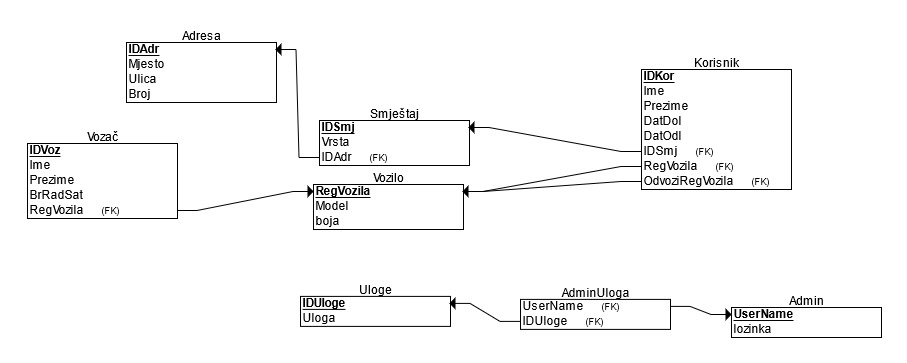
\includegraphics[width=\linewidth]{slike/DentAll_RelacijskiDijagramBaze.png}
				\centering
				\caption{Dijagram baze podataka}
				\label{fig:dijagramBaze}
			\end{figure}
			\eject
			
		\section{Dijagram razreda}
		
			{Na sljedećim slikama prikazani su dijagrami razreda koji se odnose na \textit{backend} dio aplikacije. Na slici 4.1 prikazan je cjelokupni dijagram razreda, a na ostalima su razdvojeni u smislene cjeline. U implementaciji korištena je \textit{Spring Boot} tehnologija. Postoje tri sloja aplikacije: \textit{Controller}(REST API), \textit{Service}(poslovna logika) te \textit{Repository}(pristup podacima). }\\
			
			\begin{figure}[H]
				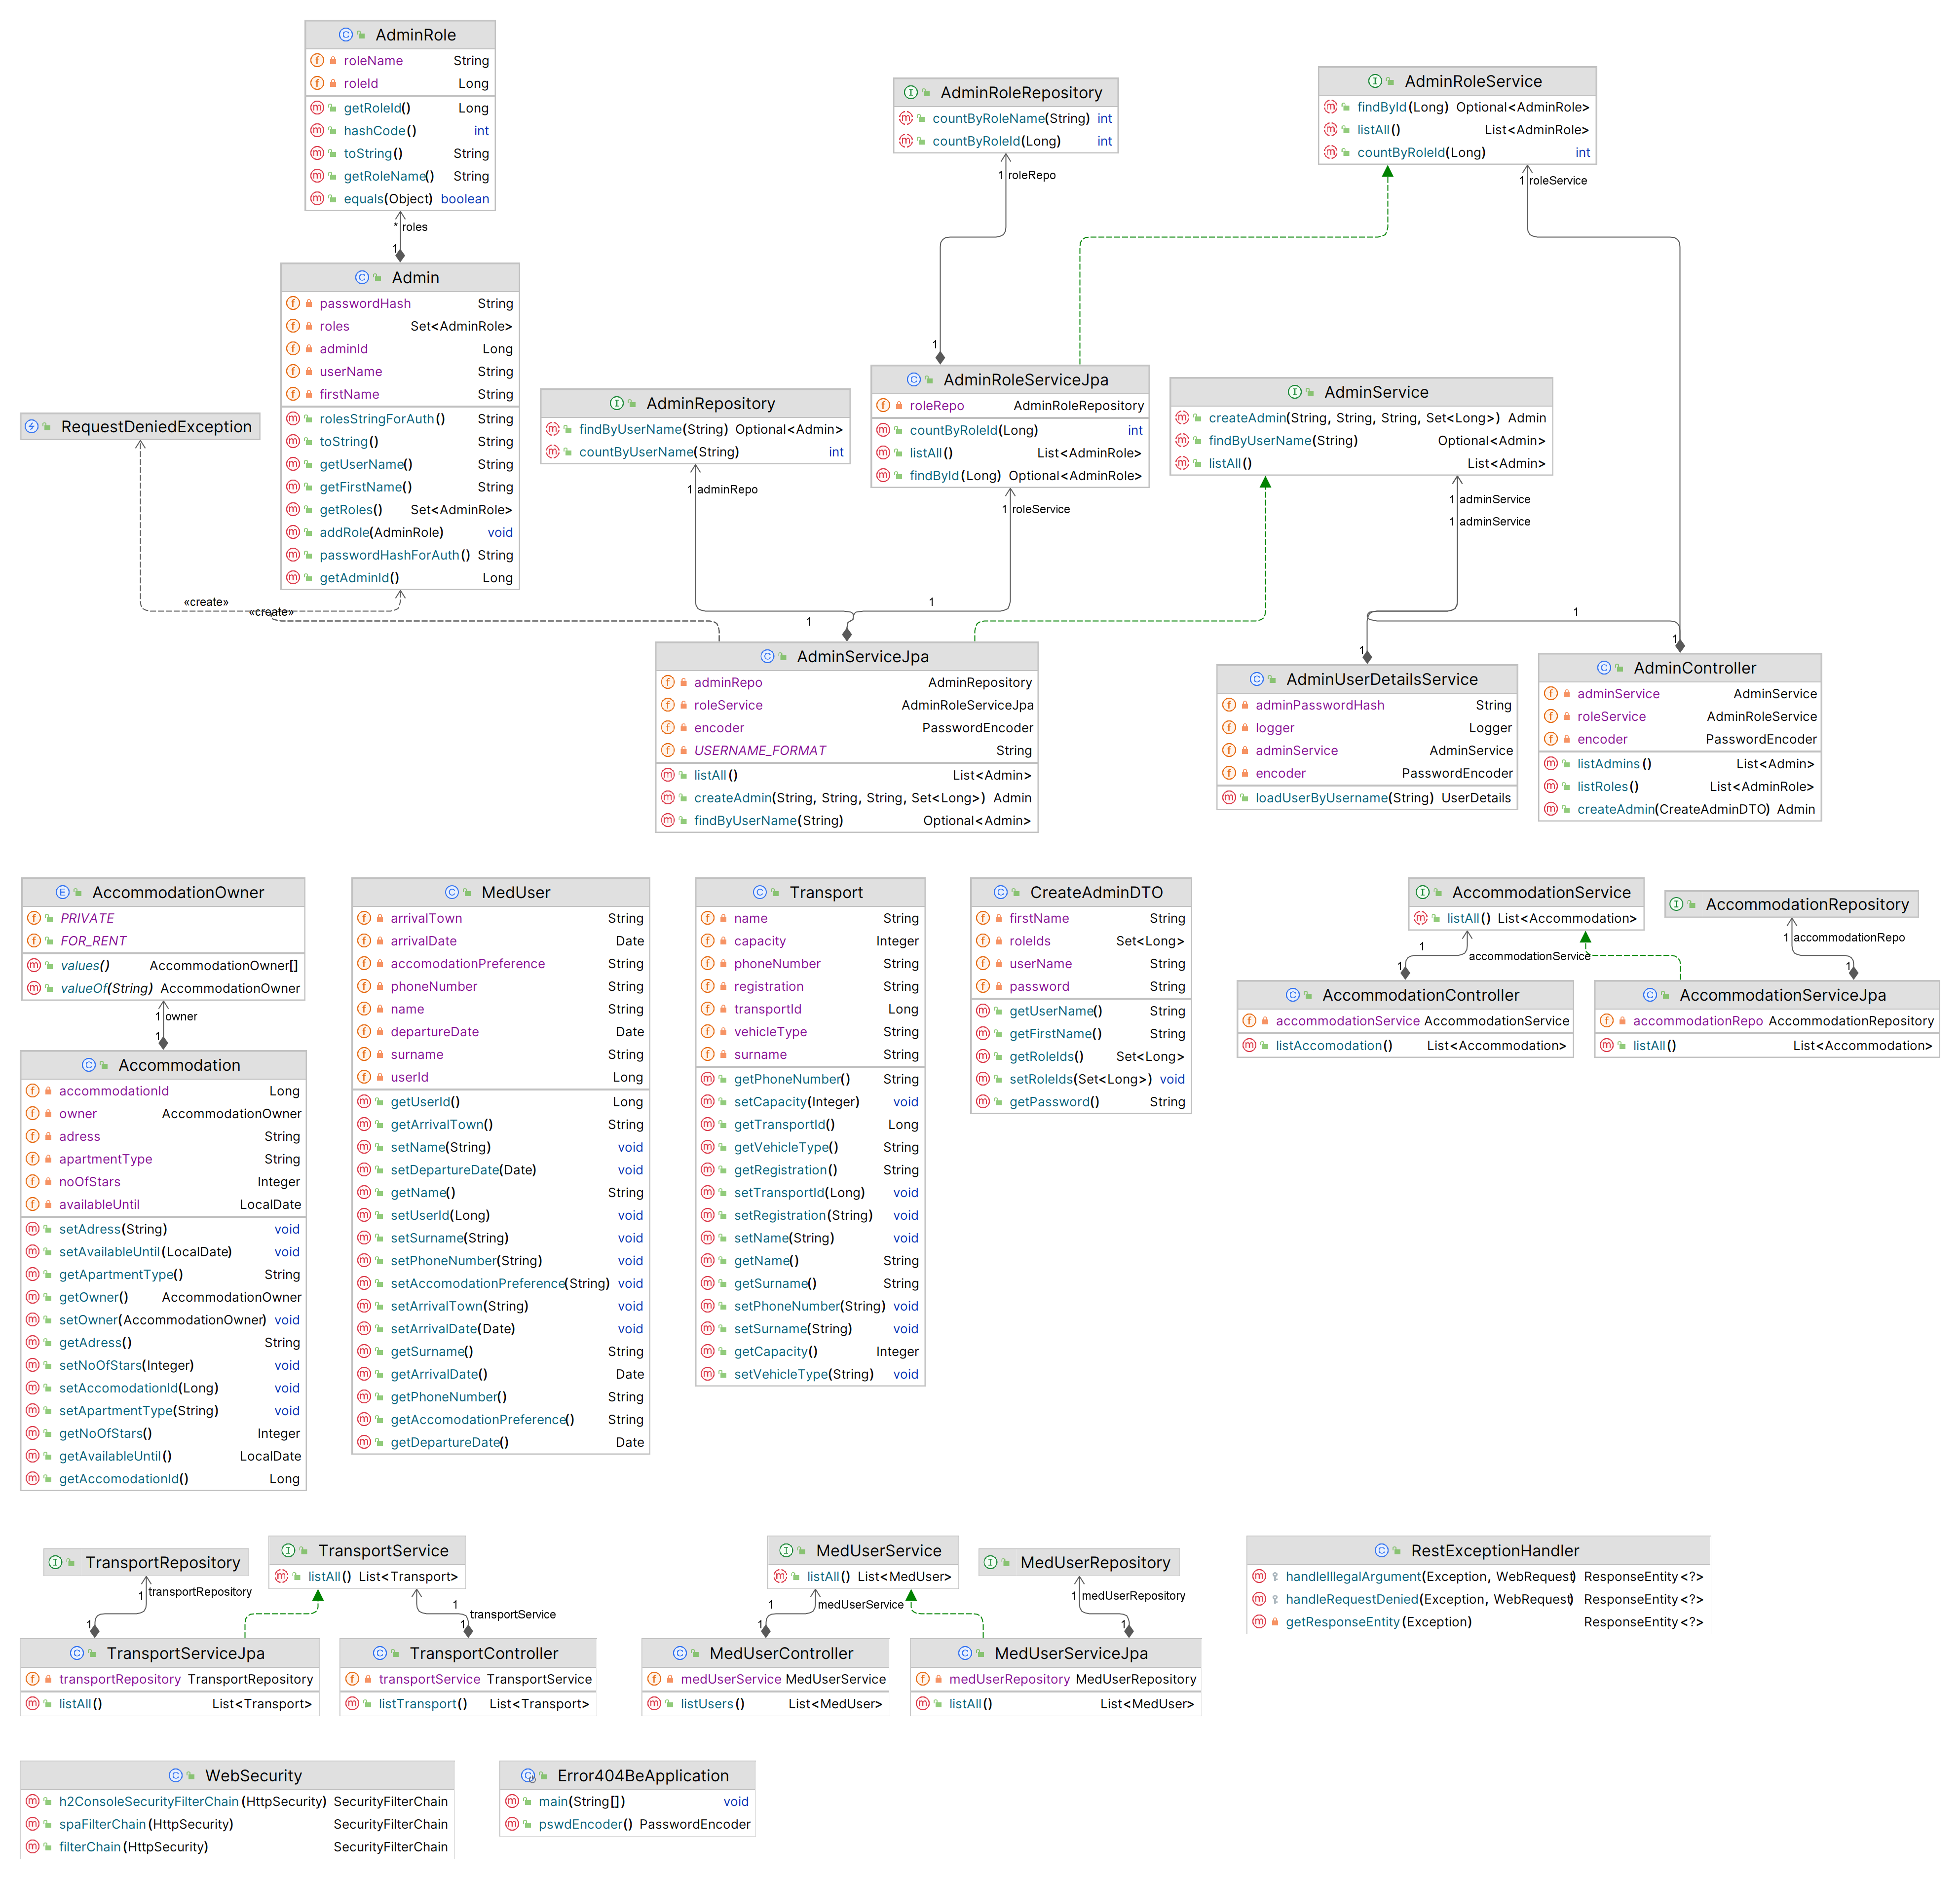
\includegraphics[width=\textwidth]{slike/CjelokupanDijagramRazreda.PNG}
				\caption{Cjelokupan dijagram razreda}
				\label{classDiagram}
			\end{figure}
			
			\begin{figure}[H]
				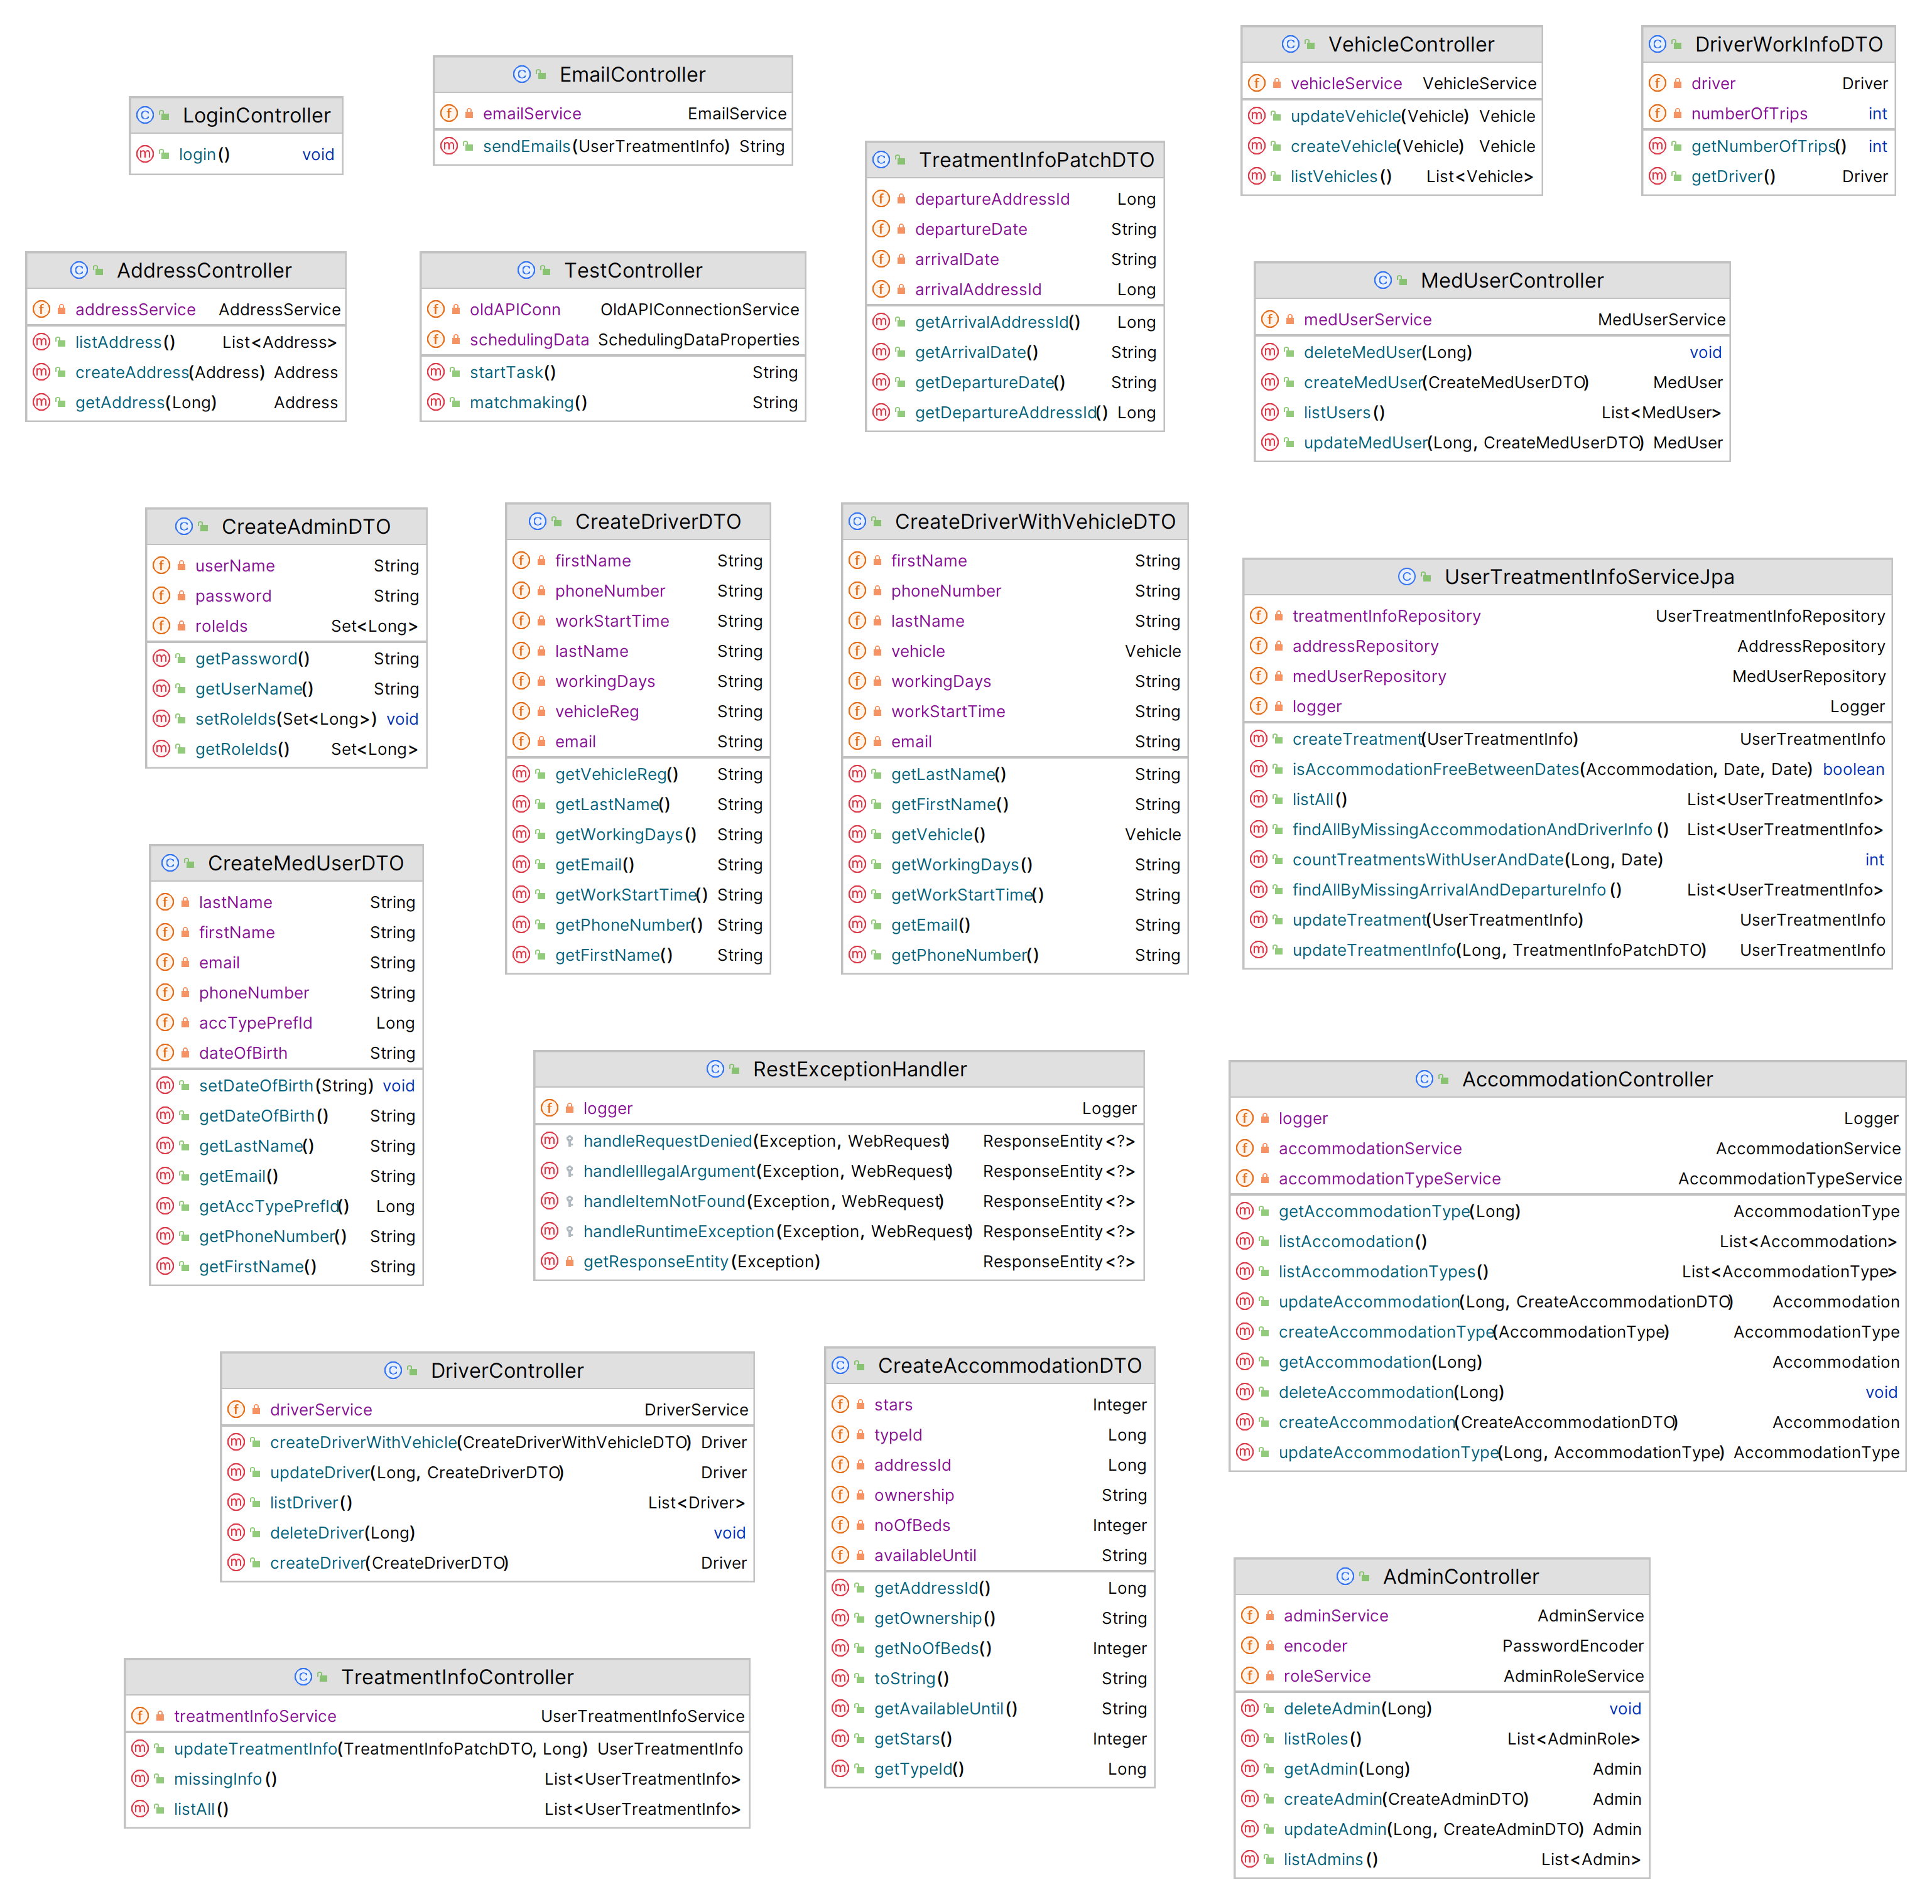
\includegraphics[width=\textwidth]{slike/rest.PNG}
				\caption{Dijagram razreda - Controller}
				\label{restDiagram}
			\end{figure}
			
			{Navedene klase nasljeđuju REST Controller koji je zadužen za rukovanje HTTP zahtjevima i za pružanje odgovarajućih odgovora. REST Controller vraća podatke u JSON formatu. \\ 
			CreateAdminDTO je \textit{Data transfer Object} koji je zadužen za stvaranje administratora. \textit{DTO} služi za transfer podataka između slojeva aplikacije, pogotovo između klijenta i servera. \\
			AdminUserDetailsService je \textit{Spring service} komponenta koja služi za baratanje detaljima administratora tijekom prijave i prilagođavanje korisničkih detalja na temelju odgovarajućih uloga i vjerodajnica, te osiguravanje sigurnosti}\\
			
			\begin{figure}[H]
				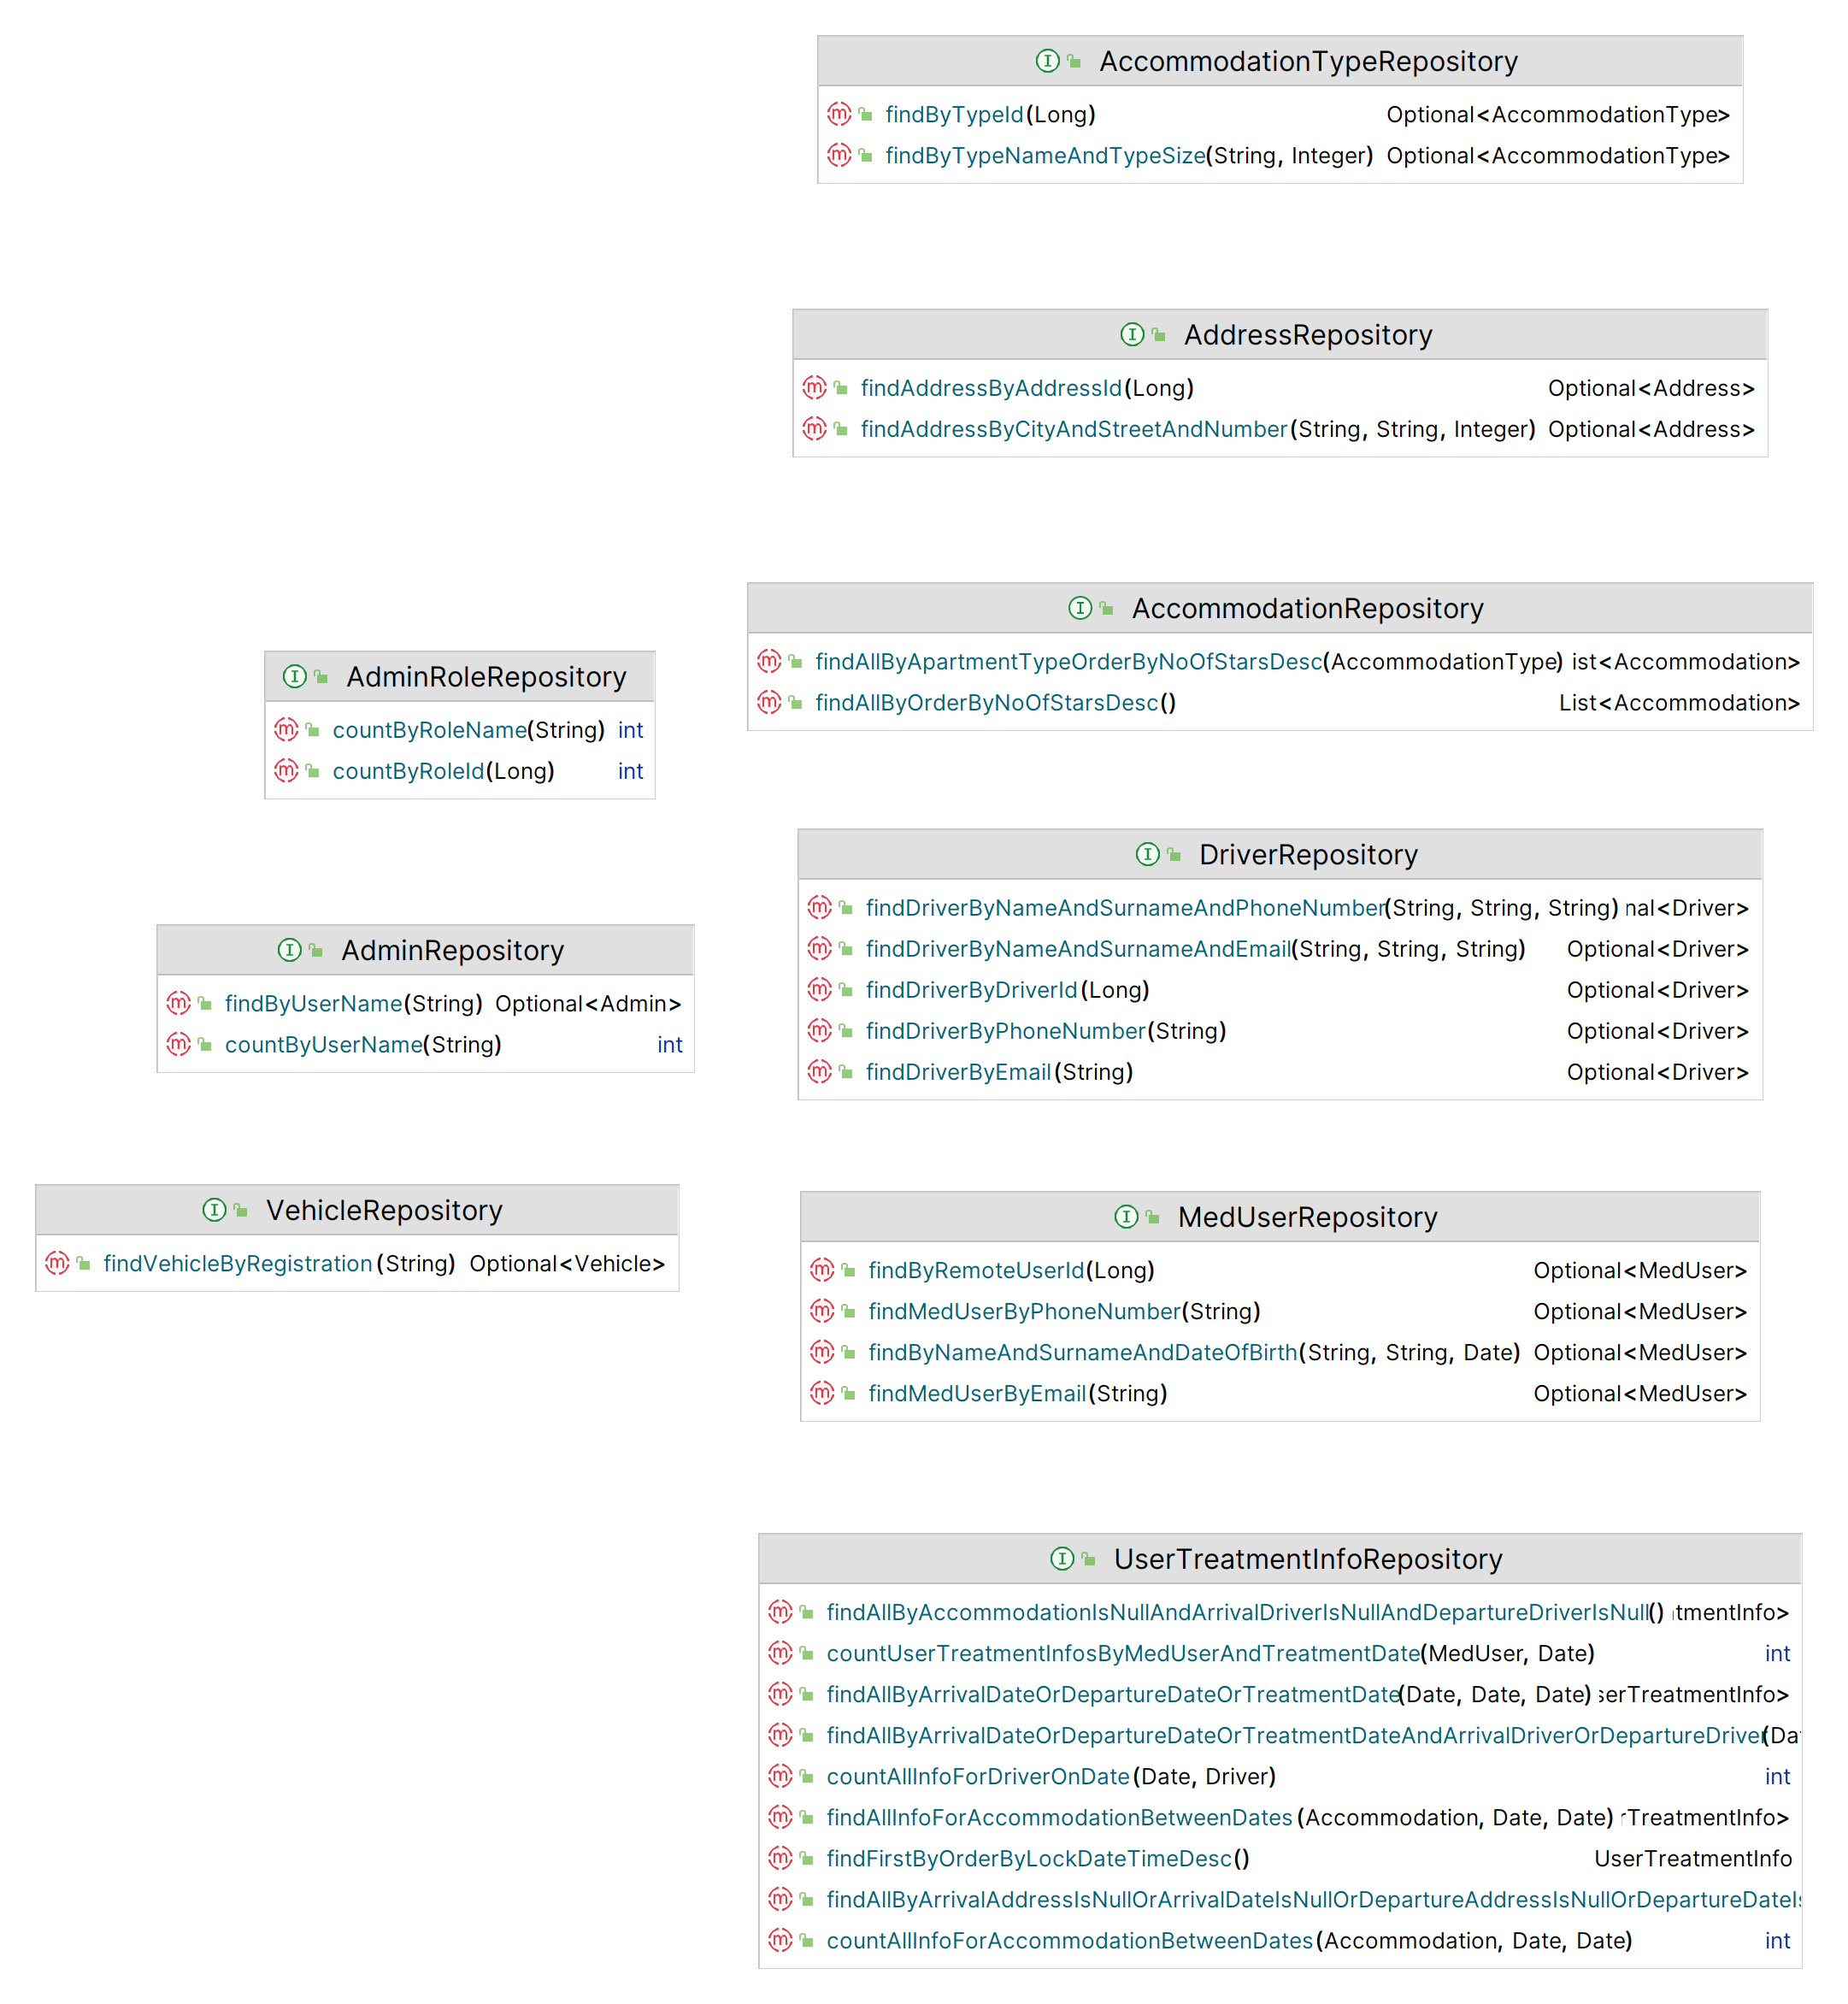
\includegraphics[width=\textwidth]{slike/dao.PNG}
				\caption{Dijagram razreda - Repository}
				\label{repositoryDiagram}
			\end{figure}
			
			{Navedena sučelja nasljeđuju \textit{JPARepository} koji pruža generičke metode za operacije s podatcima, poput spremanja, ažuriranja, brisanja i slično.}\\
			
			\begin{figure}[H]
				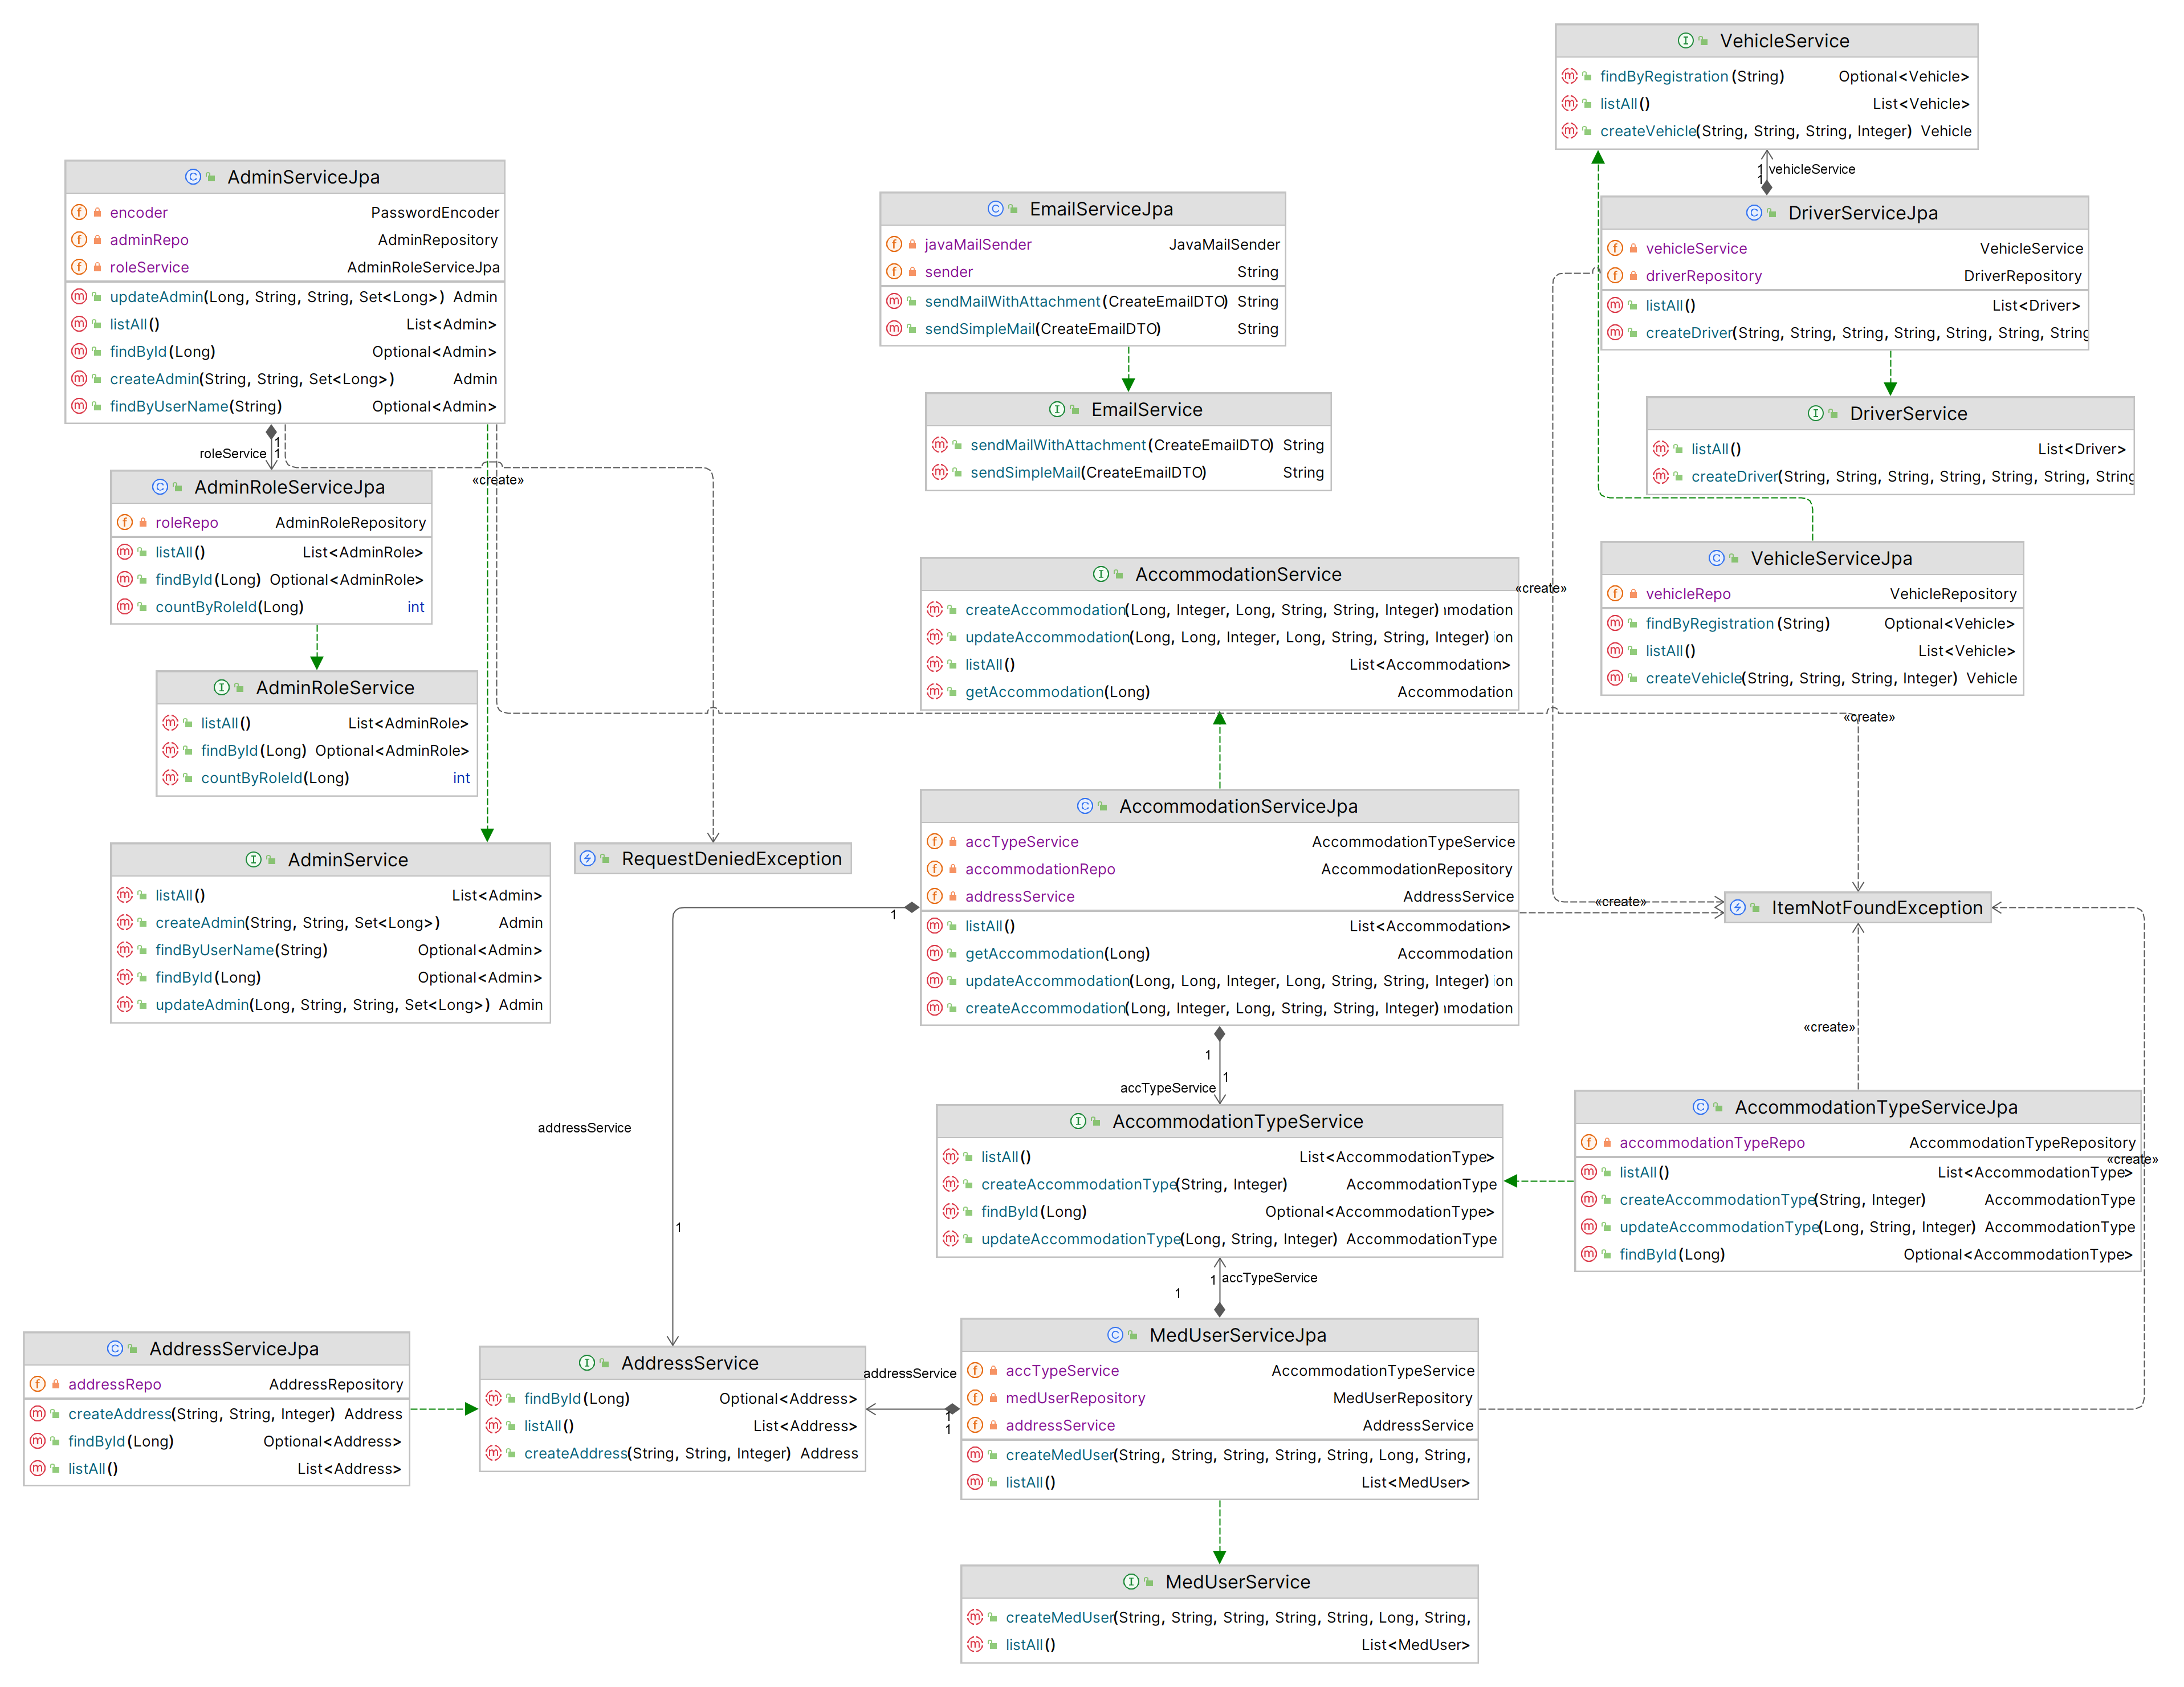
\includegraphics[width=\textwidth]{slike/service.PNG}
				\caption{Dijagram razreda - Service}
				\label{serviceDiagram}
			\end{figure}
			
			{Navedene \textit{Service} klase su \textit{Spring Service} klase, sadrže poslovnu logiku aplikacije, tj. odgovorni su za obradu podataka, implementaciju algoritama itd. Ponašaju se kao sloj između \textit{Controllera} i \textit{Repositoryja}.\\
			\textit{AdminService} sadrži metodu \textit{createAdmin} za stvaranje administratora. Postoji provjera raznih svojstava, poput duljine lozinke, duljine nadimka, postoji li već neki administrator s tim nadimkom, postojanje navedenih uloga itd. Ako je sve uspješno sprema se novi administrator u \textit{AdminRepository}.}\\
			
			\begin{figure}[H]
				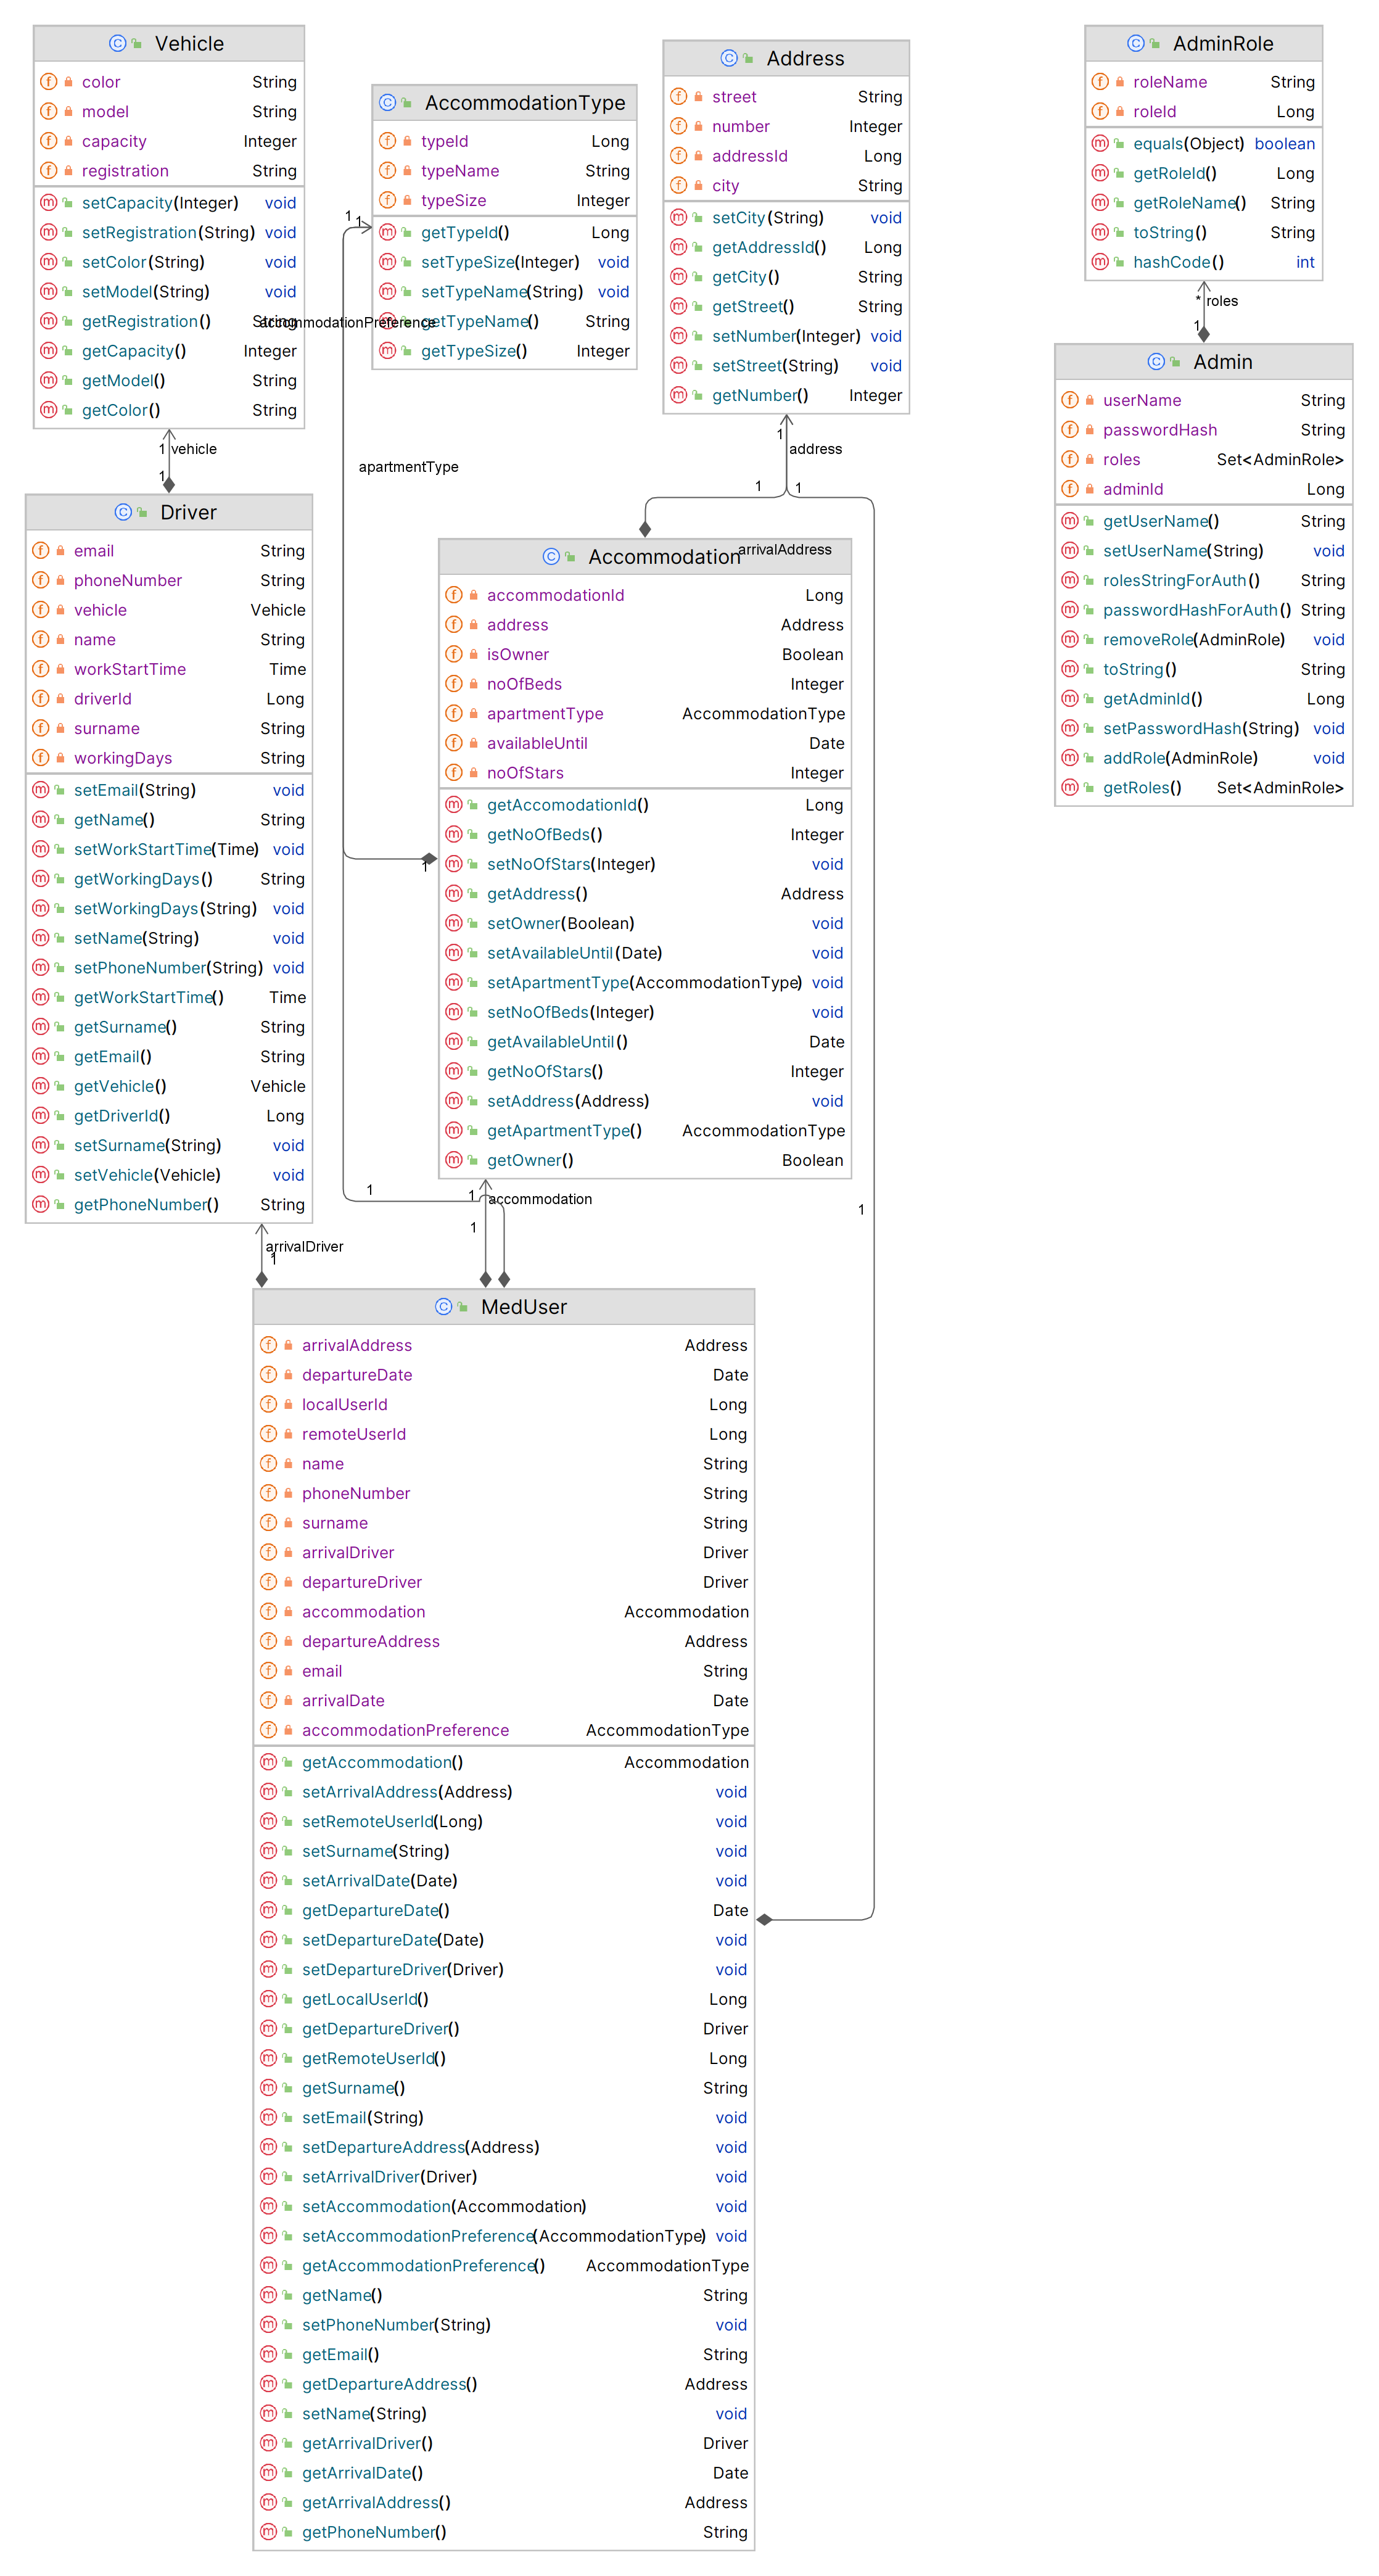
\includegraphics[width=\textwidth]{slike/domain.PNG}
				\caption{Dijagram razreda - Models}
				\label{domainDiagram}
			\end{figure}
			
			{Modeli predstavljaju strukturu baze podataka u našoj aplikaciji. Tako imamo klase: \textit{Admin, MedUser, Accomomodation te Transport} sa svojim privatnim atributima te javnim metodama. Tako na primjer \textit{Admin} ima svoj ID, nadimak, ime te pripadajuće uloge, koje mogu biti smještajni administrator(ima najveće ovlasti), korisnički administrator te prijevozni administrator, što je sadržano u enumeraciji \textit{AdminRole}. \textit{Accommodation} i \textit{Transport} sadrže sve podatke vezane uz smještaj, odnosno prijevoz, a \textit{MedUser} sadrži sve potrebno za definiranje korisnika medicinskih usluga. }\\
			
			
			
			%\textbf{\textit{dio 2. revizije}}\\			
			
			%\textit{Prilikom druge predaje projekta dijagram razreda i opisi moraju odgovarati stvarnom stanju implementacije}
			
			
			
			\eject
		
		\section{Dijagram stanja}
			
			{Na slici 4.7 prikazan je dijagram stanja. Prvo na što admin naiđe je prijava, te nakon toga mu se prikaže web stranica za admina. Na toj stranici može odabrati opciju pregleda svih unesenih podataka te izbrisati ili promijeniti iste. Ako je admin prijavljen kao korisnički admin onda on odabirom opcije za 
			dodavanje novog korisnika može dodati novog korisnika. Dok ako je admin prijavljen kao admin prijevoza, može dodavati nove prijevoznike. Smještajni admin može odabirom opcije za dodavanje novog administratora, dodati novog administratora, ali isto tako odabirom opcije za dodavanje novog smještaja, može dodati novi smještaj.  }
			
			\begin{figure}[H]
				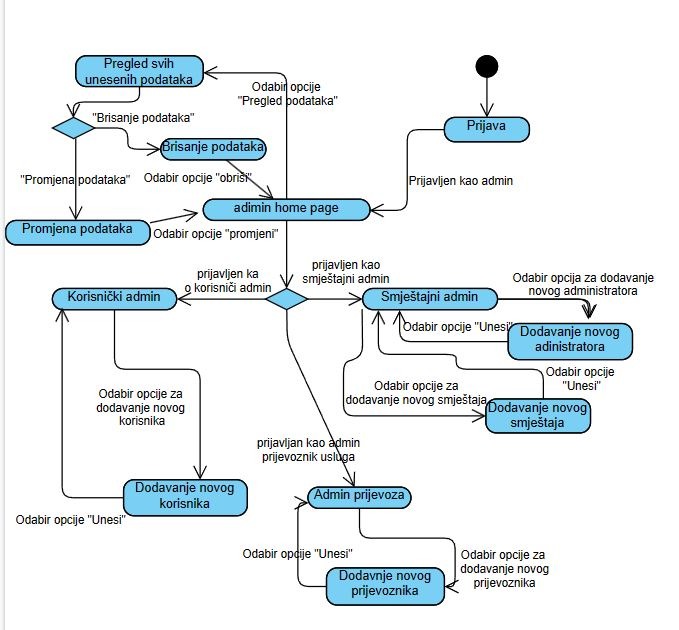
\includegraphics[width=\linewidth]{slike/Dijagram stanja.JPG}
				\centering
				\caption{Dijagram stanja}
				\label{fig:Dijagram stanja}
			\end{figure}

			%\textbf{\textit{dio 2. revizije}}\\
			
			%\textit{Potrebno je priložiti dijagram stanja i opisati ga. Dovoljan je jedan dijagram stanja koji prikazuje \textbf{značajan dio funkcionalnosti} sustava. Na primjer, stanja korisničkog sučelja i tijek korištenja neke ključne funkcionalnosti jesu značajan dio sustava, a registracija i prijava nisu. }
			
			
			\eject 
		
		\section{Dijagram aktivnosti}

		{Na slici 4.8 prikaza je dijagram aktivnosti. Sve počinje prijavom. Uneseno korisničko ime i lozinka se provjeravaju s bazom podataka. Ako je neispravna prijava, admin se vrača na obrazac za unos podataka za prijavu, dok ako je prijava uspješna, pojavljuje se prikaz vrsta admina.
		Ako je prijavljen korisnički admin, on može dodavati nove korisnike. Adim prijevoza može dodavati nove prijevoznike. Dok smještajni admin može dodavati novi smještaj te dodavati nove admine.}
			
		\begin{figure}[H]
			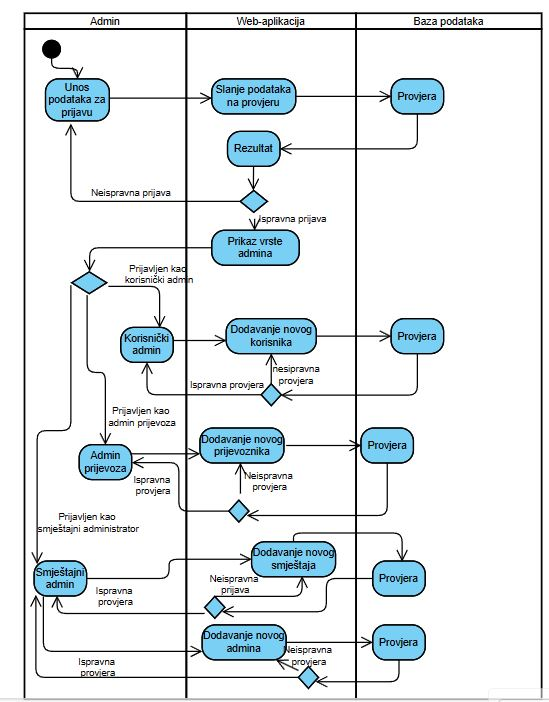
\includegraphics[width=\linewidth]{slike/Dijagram aktivnsti.JPG}
			\centering
			\caption{Dijagram aktivnosti}
			\label{fig:Dijagram aktivnosti}
		\end{figure}


			%\textbf{\textit{dio 2. revizije}}\\
			
			 %\textit{Potrebno je priložiti dijagram aktivnosti s pripadajućim opisom. Dijagram aktivnosti treba prikazivati značajan dio sustava.}
			
			\eject
		\section{Dijagram komponenti}

		{Na slici 4.9 prikazan je dijagram komponenti koji pokazuje međuovisnosti između frontenda, backenda i baze podataka. Frontend ima poseban server za HTML, CSS i JS datoteke koje služe za strukturu i dizajn web stranice. REST API komponenti pristupa se preko sučelja za dohvat JSON podataka te poslužuje podatke backendu. 
		Cijeli backend je napravljen na Springu te backend komunicira s bazom podataka slanjem SQL upita.}
		
			\begin{figure}[H]
				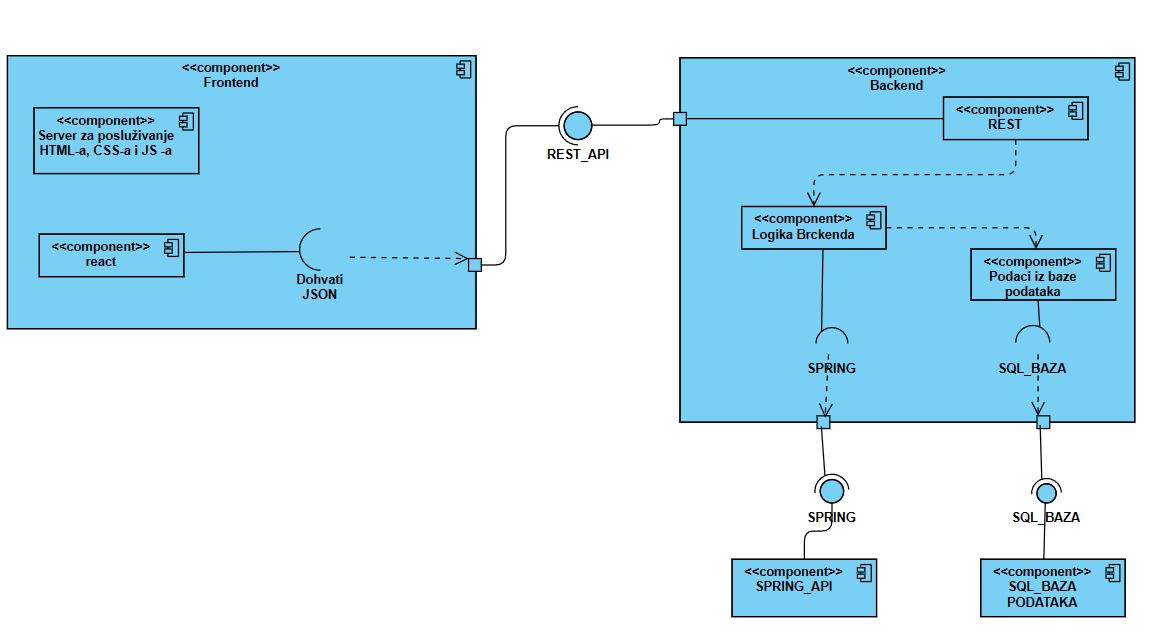
\includegraphics[width=\linewidth]{slike/dijagram komponenti.JPG}
				\centering
				\caption{Dijagram komponenti}
				\label{fig:Dijagram komponenti}
			\end{figure}			%\textbf{\textit{dio 2. revizije}}\\
		
			 %\textit{Potrebno je priložiti dijagram komponenti s pripadajućim opisom. Dijagram komponenti treba prikazivati strukturu cijele aplikacije.}